\documentclass[12pt]{report}

\usepackage{booktabs}
\usepackage{float}
\usepackage{array}
\usepackage[export]{adjustbox}
\usepackage{amsmath}
\usepackage{amssymb}
\usepackage{fancyhdr}
\usepackage{verbatim}
\usepackage{graphicx}
\graphicspath{ {imgs/} }

%\setlength{\topmargin}{-.3 in}
%\setlength{\oddsidemargin}{0in}
%\setlength{\evensidemargin}{0in}
%\setlength{\textheight}{9.in}
%\setlength{\textwidth}{6.5in}

\pagestyle{fancy}
\fancyhead[L]{Zhihao Ai}
\fancyhead[C]{Homework 5}
\fancyhead[R]{CS 422}

%opening
\title{CS 422 Data Mining\\
Homework 5}
\author{Zhihao Ai}
\date{}

%custom commands
\newcommand{\ds}{\displaystyle}

\newcolumntype{C}{ >{\centering\arraybackslash} m{2.5em} }

\begin{document}

\maketitle
\newpage

\section*{Recitation Problems}
\begin{enumerate}
	\item [\textbf{4}]
	\begin{enumerate}
		\item
		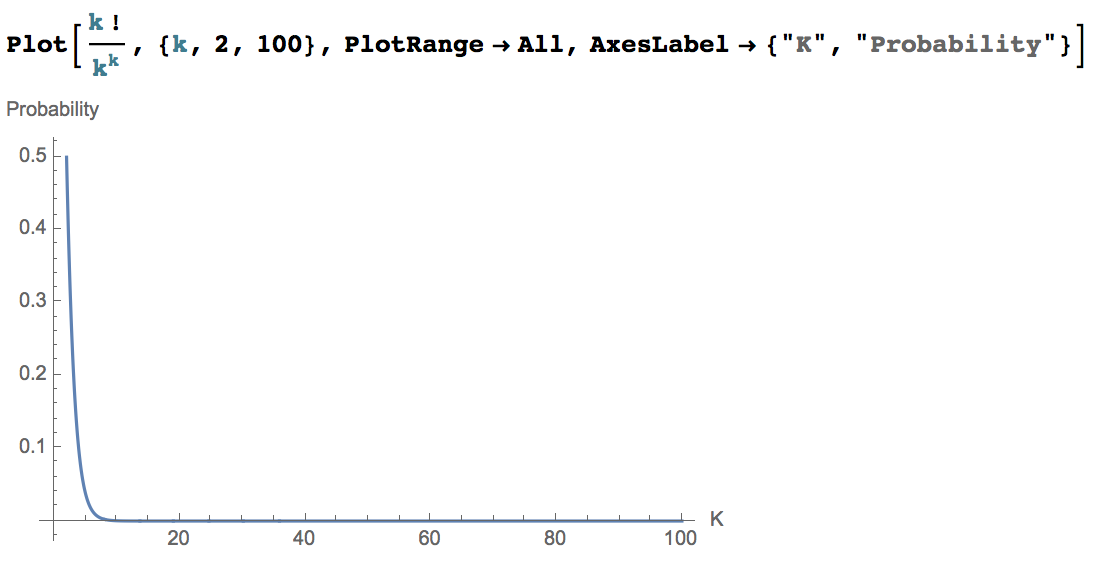
\includegraphics[scale=0.5, valign=t]{4a.png}
		
		\item 
		\begin{flalign*}
		&p = (1 - (1 - 1/K)^{2K})^K &\\
		&p_{K=10} = (1 - (1 - 1/10)^{20})^{10} \approx 0.274 &\\
		&p_{K=100} = (1 - (1 - 1/100)^{200})^{100} \approx 5.66 \times 10^{-7} &\\
		&p_{K=1000} = (1 - (1 - 1/1000)^{2000})^{1000} \approx 8.24 \times 10^{-64}&
		\end{flalign*}
	\end{enumerate}

	\item [\textbf{7}]
	Suppose each region is allocated one single centroid, the SSE of the denser region would be smaller than that of the less dense region since the points in the denser region are more ``closer" to the  centroid. Thus, by adding more centroids to both regions, the decrease of SSE of the less dense region would be greater than that of the denser region. Therefore, more centroids should be allocated to the less dense region as (b) states.
	
	\item [\textbf{11}]
	\begin{enumerate}
		\item 
		If the SSE of one attribute is low for all clusters, the values of the attribute for all instances are approximately the same.
		\item 
		If the SSE of one attribute is low for just one cluster, the cluster is well distinguished by this attribute.
		\item 
		If the SSE of an attribute is high for all clusters, the attribute is probably noise.
		\item 
		If the SSE of an attribute is high for just one cluster, the cluster is not well defined by this attribute.
		\item 
		We should try to eliminate those attributes for which the SSE is low or high for all clusters.
	\end{enumerate}

	\item [\textbf{16}]
	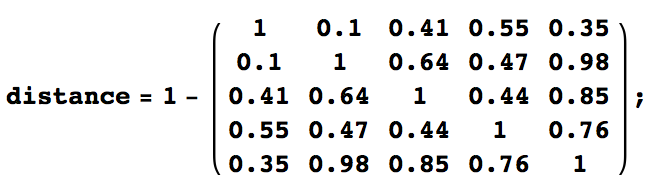
\includegraphics[scale=0.7,valign=t]{16.png}
	\begin{enumerate}
		\item Single link:\\
		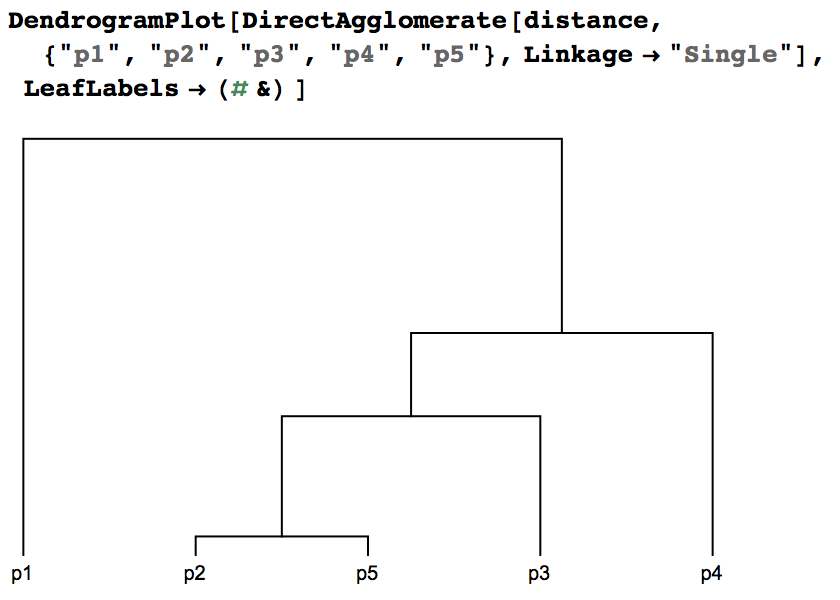
\includegraphics[scale=0.7,valign=t]{16a.png}
		
		\item Complete link:\\
		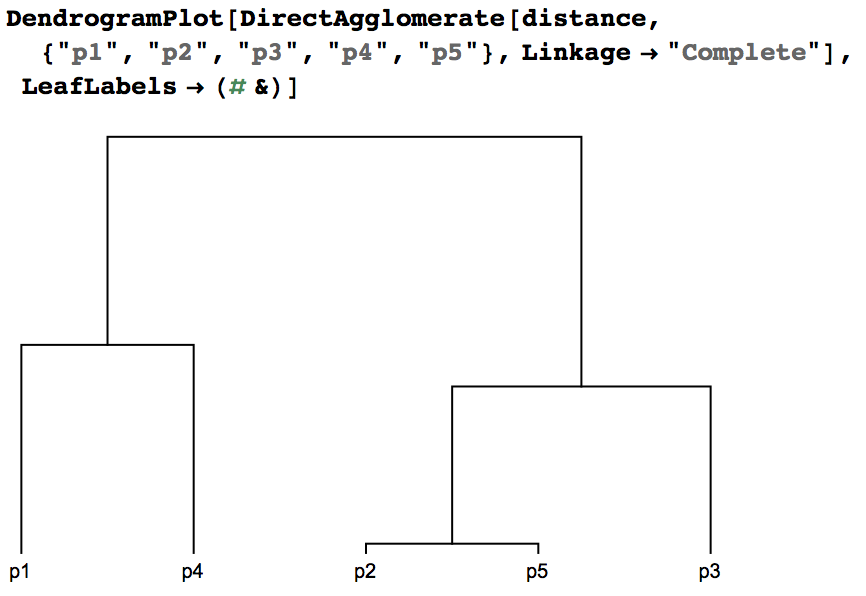
\includegraphics[scale=0.7,valign=t]{16b.png}
	\end{enumerate}

	\item [\textbf{17}]
	\begin{enumerate}
		\item 
		\begin{enumerate}
			\item
			\begin{tabular}{m{5em}*{7}{c}} \toprule
				$dist(\mathbf{c}_i, \mathbf{x})$ & 6 & 12 & 18 & 24 & 30 & 42 & 48 \\ \midrule
				$\mathbf{c}_1 = 18$ & 12 & 6 & 0 & 6 & 12 & 24 & 30 \\ 
				$\mathbf{c}_2 = 45$ & 39 & 33 & 27 & 21 & 15 & 3 & 3 \\ \bottomrule
			\end{tabular}
			\medbreak
			\(\ds
			C_1 = \{6, 12, 18, 24, 30\}\\
			\text{SSE}_{C_1} = \sum_{\mathbf{x}\in C_1} dist(\mathbf{c}_i, \mathbf{x})^2 = 12^2+6^2+0^2+6^2+12^2 = 360\\
			C_2 = \{42, 48\}\\
			\text{SSE}_{C_2} = \sum_{\mathbf{x}\in C_2} dist(\mathbf{c}_i, \mathbf{x})^2 = 3^2+3^2 = 18\\
			\text{Total SSE} = \sum_{i=1}^{K} \sum_{\mathbf{x}\in C_i} dist(\mathbf{c}_i, \mathbf{x})^2 = 360 + 18 = 378
			\)
			
			\item
			\begin{tabular}{m{5em}*{7}{c}} \toprule
				$dist(\mathbf{c}_i, \mathbf{x})$ & 6 & 12 & 18 & 24 & 30 & 42 & 48 \\ \midrule
				$\mathbf{c}_1 = 15$ & 9 & 3 & 3 & 9 & 15 & 27 & 33 \\ 
				$\mathbf{c}_2 = 40$ & 34 & 28 & 22 & 16 & 10 & 2 & 8 \\ \bottomrule
			\end{tabular}
			\medbreak
			\(\ds
			C_1 = \{6, 12, 18, 24\}\\
			\text{SSE}_{C_1} = \sum_{\mathbf{x}\in C_1} dist(\mathbf{c}_i, \mathbf{x})^2 = 9^2+3^2+3^2+9^2 = 180\\
			C_2 = \{30, 42, 48\}\\
			\text{SSE}_{C_2} = \sum_{\mathbf{x}\in C_2} dist(\mathbf{c}_i, \mathbf{x})^2 = 10^2+2^2+8^2 = 168\\
			\text{Total SSE} = \sum_{i=1}^{K} \sum_{\mathbf{x}\in C_i} dist(\mathbf{c}_i, \mathbf{x})^2 = 180 + 168 = 348
			\)
		\end{enumerate}
	
		\item 
		\begin{enumerate}
			\item 
			\(\ds
			\mathbf{c}'_1 = \frac{1}{m_1} \sum_{\mathbf{x}\in C_1} \mathbf{x} = \frac{6+12+18+24+30}{5} = 18 = \mathbf{c}_1\\
			\mathbf{c}'_2 = \frac{1}{m_2} \sum_{\mathbf{x}\in C_2} \mathbf{x} = \frac{42+48}{2} = 45 = \mathbf{c}_2
			\)
			
			\item 
			\(\ds
			\mathbf{c}'_1 = \frac{1}{m_1} \sum_{\mathbf{x}\in C_1} \mathbf{x} = \frac{6+12+18+24}{4} = 15 = \mathbf{c}_1\\
			\mathbf{c}'_2 = \frac{1}{m_2} \sum_{\mathbf{x}\in C_2} \mathbf{x} = \frac{30+42+48}{3} = 40 = \mathbf{c}_2
			\)
		\end{enumerate}
		Since the centroids remain unchanged, both sets of centroids represent stable solutions.
		
		\item 
		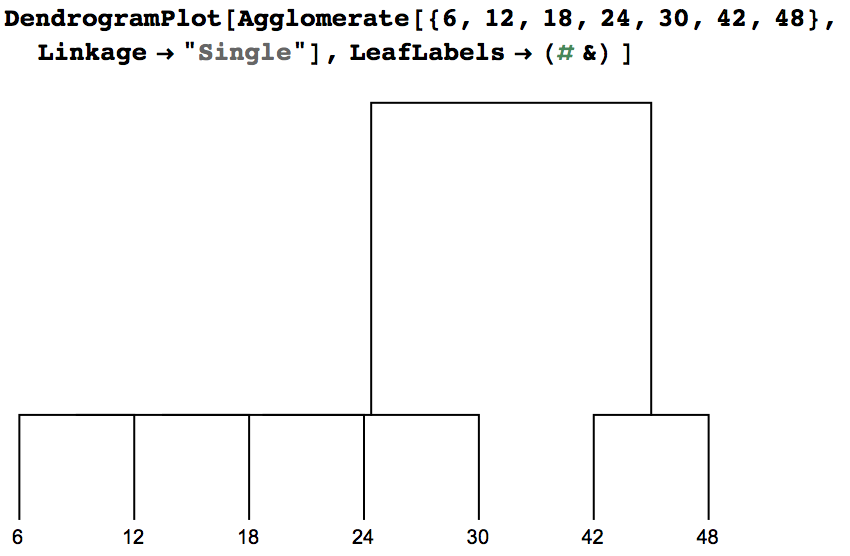
\includegraphics[scale=0.7,valign=t]{17c.png}\\
		Therefore, $\{6, 12, 18, 24, 30\}$ and $\{42, 48\}$ are the two clusters produced by single link.
		
		\item 
		K-means produces clusters with minimum SSE when $\mathbf{c}_1 = 15, \mathbf{c}_2 = 40$, but these two centroids are not the centers of ``most natural" clusters of which the  centroids are $\mathbf{c}_1 = 18, \mathbf{c}_2 = 45$. So, single link seems to produce the ``most natural" clustering in this situation.
		
		\item 
		This natural clustering is center-based and contiguous.
		
		\item 
		K-means finds clusters of equal size. Since its objective is to minimize SSE, in our case, it breaks $\{6, 12, 18, 24, 30\}$ to form smaller clusters so that SSE is reduced.
	\end{enumerate}

	\item [\textbf{21}]
	Entropy:
	\begin{align*}
	p_{ij} &= \frac{m_{ij}}{m_i}\\
	e_i &= -\sum_{j=1}^L p_{ij} \log_2 p_{ij}\\
	entropy &= \sum_{i=1}^K \frac{m_i}{m}e_i
	\end{align*}
	Purity:
	\begin{align*}
	p_i &= \max_j{p_{ij}}\\
	purity &= \sum_{i=1}^K \frac{m_i}{m} p_i
	\end{align*}
	In mathematica:\\
	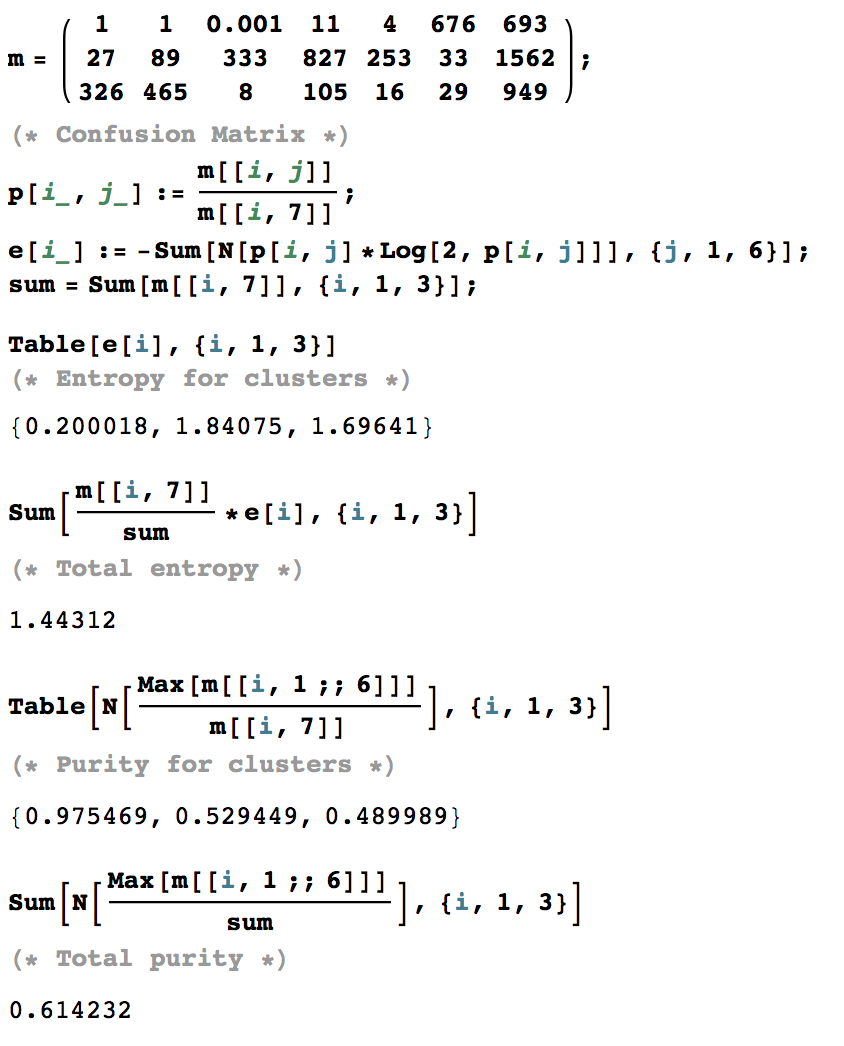
\includegraphics[width=\linewidth]{21.png}
	\begin{table}[H]
		\centering
		\begin{tabular}{m{3.5em} cc}
			\toprule
			Cluster & Entropy & Purity \\ \midrule
			\#1     & 0.20    &  0.98  \\ \midrule
			\#2     & 1.84    &  0.53  \\ \midrule
			\#3     & 1.70    &  0.49  \\ \midrule
			Total   & 1.44    &  0.61  \\ \bottomrule
		\end{tabular}
	\end{table}
	
	\item [\textbf{22}]
	\begin{enumerate}
		\item 
		Yes. The uniformly spaced points will have equal density throughout the unit square since the space between one another is equal, while the points generated from a uniform distribution will have regions of various densities.
		\item 
		The set of points generated from a uniform distribution.
		\item 
		For the uniform data set, depending on the threshold, DBSCAN would count all points as one single cluster or all noise.\\
		For the random data set, since the density varies, DBSCAN would typically find clusters.
	\end{enumerate}
	
	\item [\textbf{23}]
	Distance matrix:
	\begin{table}[H]
		\centering
		\begin{tabular}{*{5}{C}}
			\toprule
			   &  P1  &  P2  &  P3  &  P4  \\ \midrule
			P1 &  0   & 0.10 & 0.65 & 0.55 \\ \midrule
			P2 & 0.10 &  0   & 0.70 & 0.60 \\ \midrule
			P3 & 0.65 & 0.70 &  0   & 0.30 \\ \midrule
			P4 & 0.55 & 0.60 & 0.30 &  0   \\ \bottomrule
		\end{tabular}
	\end{table}
	Silhouette coefficient for $P_i$ is given by \(s_i = (b_i - a_i)/\max(a_i, b_i) \)\\
	\(
		s_1 = (0.6-0.1)/0.6 \approx 0.833\\
		s_2 = (0.65-0.1)/0.65 \approx 0.846\\
		s_3 = (0.675-0.3)/0.675 \approx 0.556\\
		s_4 = (0.575-0.3)/0.575 \approx 0.478\\
		s_{c1} = (0.833+0.846)/2 \approx 0.840\\
		s_{c2} = (0.556+0.478)/2 = 0.517\\
		s = (0.8395+0.517)/2 \approx 0.679
	\)
\end{enumerate}

\section*{Practicum  Problems}
\subsection*{Problem 1}
\begin{figure}[H]
	\centering
	\includegraphics[width=\linewidth]{p1dist.png}
\end{figure}
The data labeled 3 are all assigned to $C1$; those labeled 2 are mostly assigned to $C2$; those labeled 1 are more likely to be assigned to $C1$, but some of them are instead assigned to $C2$ or $C3$.\\
As shown in the figure, the probabilities are 
\begin{table}[H]
	\centering
	\begin{tabular}{>$c<$ >$c<$ >$c<$ >$c<$}
		\toprule
		   & origin=1      & origin=2      & origin=3 \\ \midrule
		C1 & 0.482\pm0.062 & 0.957\pm0.047 & 1        \\ \midrule
		C2 & 0.261\pm0.055 & 0.043\pm0.047 & 0        \\ \midrule
		C3 & 0.257\pm0.054 & 0             & 0        \\ \bottomrule
	\end{tabular}
\end{table}
Changing the \textbf{Max Depth} does not affect the results, since in the hierarchical clustering, merging decisions are final and by selecting the top 3 clusters, we are always ``cutting" the dendrogram tree at level 2, which results in 3 clusters. So whatever max depth we set ($\ge 2$ since we want to find 3 clusters), the three final clusters we have is always the same.

\subsection*{Problem 2}

\end{document}
